%%%%%%%%%%%%%%%%%%%%%%%%%%%%%%%%%%%%%%%%%
% Beamer Presentation
% Standard LaTeX Template used for creating presentation of Firebird-V Robot and other tutorials. 
% Author: Saurav Shandilya (e-Yantra Team)
% Reference: www.LaTeXTemplates.com Version 1.0 (10/11/12)
%
%%%%%%%%%%%%%%%%%%%%%%%%%%%%%%%%%%%%%%%%%

%----------------------------------------------------------------------------------------
%	PACKAGES AND THEMES
%----------------------------------------------------------------------------------------
		
\documentclass[table,10pt,red]{beamer}	% First line -- Define document class as Beamer which is used for creating presentation using Latex
\setbeamercolor{alerted text}{fg=blue} 	% Sets color of highlighted text during presentation.  
 

% The Beamer class comes with a number of default slide themes
% which change the colors and layouts of slides. Below this is a list
% of all the themes, uncomment each in turn to see what they look like.

%\usetheme{default}
%\usetheme{AnnArbor}
%\usetheme{Antibes}
%\usetheme{Bergen}
%\usetheme{Berkeley}
\usetheme{Berlin}		%used theme in present documents.
%\usetheme{Boadilla}
%\usetheme{CambridgeUS}
%\usetheme{Copenhagen}
%\usetheme{Darmstadt}
%\usetheme{Dresden}
%\usetheme{Frankfurt}
%\usetheme{Goettingen}
%\usetheme{Hannover}
%\usetheme{Ilmenau}
%\usetheme{JuanLesPins}
%\usetheme{Luebeck}
%\usetheme{Madrid}
%\usetheme{Malmoe}
%\usetheme{Marburg}
%\usetheme{Montpellier}
%\usetheme{PaloAlto}
%\usetheme{Pittsburgh}
%\usetheme{Rochester}
%\usetheme{Singapore}
%\usetheme{Szeged}
%\usetheme{Warsaw}

% As well as themes, the Beamer class has a number of color themes
% for any slide theme. Uncomment each of these in turn to see how it
% changes the colors of your current slide theme.

%\usecolortheme{albatross}
%\usecolortheme{beaver}
%\usecolortheme{beetle}
%\usecolortheme{crane}
%\usecolortheme{dolphin}
%\usecolortheme{dove}
%\usecolortheme{fly}
%\usecolortheme{lily}
%\usecolortheme{orchid}
%\usecolortheme{rose}
%\usecolortheme{seagull}
%\usecolortheme{seahorse}
%\usecolortheme{whale}
%\usecolortheme{wolverine}

%\setbeamertemplate{footline} % To remove the footer line in all slides uncomment this line
%\setbeamertemplate{footline}[page number] % To replace the footer line in all slides with a simple slide count uncomment this line

%\setbeamertemplate{navigation symbols}{} % To remove the navigation symbols from the bottom of all slides uncomment this line
%}

%------------------------------------------------------------------------------------------
%	\usepackage is required for including various features like images, table, references etc.
%	Packages must be installed before using. These can be istalled through package manager. 
%   Various packages have dependencies and for using such packages all dependent packages must be used. 
%-----------------------------------------------------------------------------------------
\usepackage{beamerthemeshadow} % theme shadow for visual 
\usepackage{beamerthemesplit} % Creates minipage (for showing multiple images and text) on same page  
\usepackage{graphicx} % Allows including images
\usepackage{booktabs} % Allows the use of \toprule, \midrule and \bottomrule in tables
\usepackage{xcolor}
\usepackage{booktabs,array}
\usepackage{listings}
\usepackage{hyperref}	% Required for including hyperlink in document
\usepackage{verbatim,moreverb} % Required for including code snippet.
\usepackage{colortbl}
\usepackage{multirow}	% Required for creating multiple row tables
\usepackage{tikz}		% Required for drawing shapes such as circles, arrowed line, etc. 
\usetikzlibrary{arrows}
\usepackage{ragged2e}

% logo
\logo{
\includegraphics[height=1cm]{iitblogo.pdf}} % includes logo at bottom of all slides 

%----------------------------------------------------------------------------------------
%	TITLE PAGE
%----------------------------------------------------------------------------------------
% sf family, bold font
\sffamily \bfseries
% content inside [] appears at bottom of all page. content inside {} appears on first page as title. double backslash means line change 
\title
[
	e-Yantra	% bottom of all page
	\hspace{0.5cm}
	\insertframenumber/\inserttotalframenumber
]
{
	Interfacing Accelerometer MMA7361with ATmega2560 in Firebird V Robot
}

\author
[
	www.e-yantra.org 	%Name at bottom of all page 
]
% author name on title slide
{
	Shantanu Sengupta \and Chayatan \and Mukilan\\
\vspace{5mm}
  Embedded Real-Time Systems Lab\\
  Indian Institute of Technology-Bombay \\
}
\date
{
IIT Bombay \\ {\today}	%\today picks system date on title slide
}

\begin{document} % IN LATEX ALL DOCUMENT/REPORT/PRESENTATION STARTS WITH \begin{document} AND ENDS WITH \end{document}

\begin{frame}	% FRAME MEANS SLIDE. \begin{frame} STARTS THE SLIDE AND \end{frame} ENDS THE SLIDE
	\titlepage % Print the title page as the first slide
\end{frame}

% START OF SECOND SLIDE
\begin{frame}
	\frametitle{Agenda for Discussion} % Table of contents slide, comment this block out to remove it
	\tableofcontents % Throughout your presentation, if you choose to use \section{} and \subsection{} commands, these will automatically be printed on this slide as an overview of your presentation
\end{frame}

%----------------------------------------------------------------------------------------
%	PRESENTATION SLIDES
%----------------------------------------------------------------------------------------

%------------------------------------------------
\section{Accelerometer} % Sections can be created in order to organize your presentation into discrete blocks, all sections and subsections
\subsection{Introduction} % Sections can be created in order to organize your presentation into discrete blocks, all sections and subsections are automatically printed in the table of contents as an overview of the talk
%------------------------------------------------


% Start of Third slide
\begin{frame}
	\frametitle{Introduction}
 		
 		\color{black} 
\pause

			\begin{itemize}
\justifying
\item <+-|alert@+>    As the name indicates this sensor is used to measure acceleration. 
\item <+-|alert@+> Acceleration here does not mean rate of change in velocity in a particular axis but the g-force acting on the body.
\item <+-|alert@+> 	For example, an accelerometer at rest on the surface of the earth will measure an acceleration g= 9.81 m/s2 straight upwards, due to its weight. By contrast, accelerometers in free fall or at rest in outer space will measure zero.
\item <+-|alert@+> This type of acceleration that accelerometers can measure is g-force acceleration.
\end{itemize}
\end{frame}

%------------------------------------------------
\subsection{Working Principle}
\begin{frame}
	\frametitle{Working Principle}
 		\pause

\begin{minipage}[c]{0.6\textwidth}
			\begin{itemize}
\justifying
\item <+-|alert@+>  Accelerometer consists of a surface micromachined capacitive sensing cell\\ (g-cell).
\item <+-|alert@+>  This consist of a moveable plate in the center of two fixed beams such that its movement depends on the g force acting on the accelerometer.
\item <+-|alert@+>  As the center beam moves with acceleration, the distance between the beams changes and each capacitor's value will change, ($C = A \epsilon /D$). Where A is the area of the beam, $\epsilon$ is the dielectric constant, and  D is the distance between the beams.


\end{itemize}
		\end{minipage}
\begin{minipage}[c]{0.37\textwidth}
\begin{figure}
\hspace*{5mm}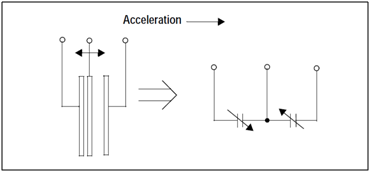
\includegraphics[width=\linewidth]{gcell.png}
\caption{Structure of a g-cell}
\end{figure}
		\end{minipage}

\end{frame}



%------------------------------------------------

\section{Interfacing of Accelerometer with FireBird V} 
\subsection{Pin Diagram} 
\begin{frame}
	\frametitle{Interfacing of Accelerometer with FireBird V}
\pause
\begin{minipage}[c]{0.60\textwidth}
\hspace*{22mm}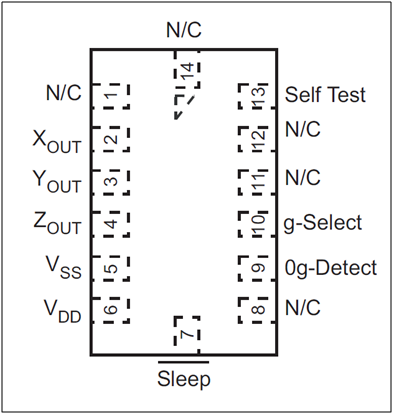
\includegraphics[width=\linewidth]{acc1.png}
		\end{minipage}
		
\end{frame}
%------------------------------------------------
\subsection{Pin Connections of MMA7361 Accelerometer} 
\begin{frame}
	\frametitle{Interfacing of Accelerometer with FireBird V}
\pause
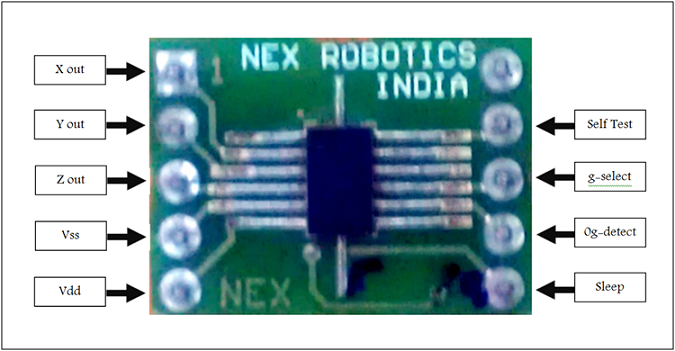
\includegraphics[width=\linewidth]{acc2.png}
		
\end{frame}
%------------------------------------------------

\subsection{Connection Details} 
 \begin{frame}
	\frametitle{Connection Details}
\pause

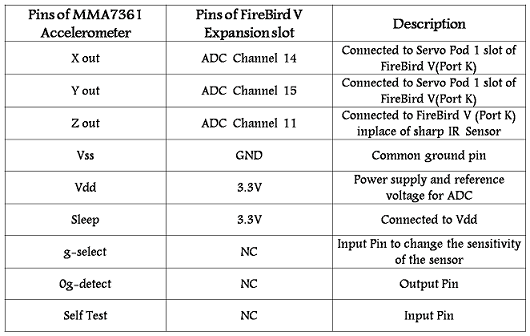
\includegraphics[width=\linewidth]{Picture1.png}
		

\end{frame}
%-------------------------------------------------------

\section{C Code} 
 \begin{frame}
	\frametitle{C Code}
\begin{center}
\huge C Code
\end{center}		

\end{frame}
%------------------------------------------------
\section{Applications using Accelerometer} 
\begin{frame}
	\frametitle{Applications using Accelerometer}
\pause
 		

\begin{minipage}[c]{0.6\textwidth}
			\begin{itemize}
\justifying
\item <+-|alert@+>  Can be used for simulating driver training.
\item <+-|alert@+>  For Robot Movement similar to the walking support system as shown in the picture to the right.
\item <+-|alert@+> Accelerometers measuring dynamic forces such as vibrations can be used for designing Virtual Keyboards



\end{itemize}
		\end{minipage}
\begin{minipage}[c]{0.37\textwidth}
\hspace*{5mm}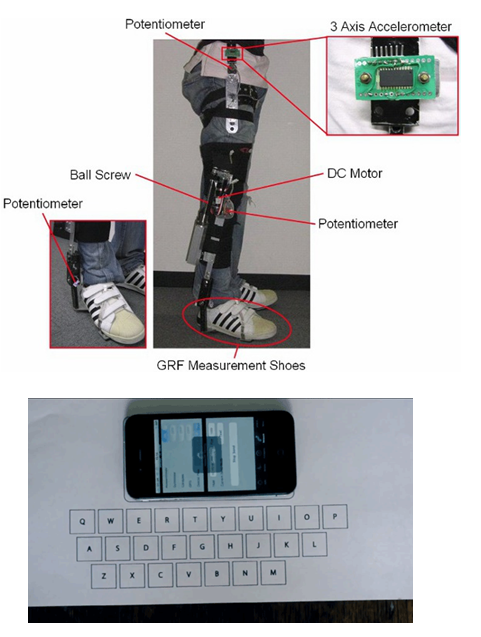
\includegraphics[width=\linewidth]{a1.png}
		\end{minipage}

\end{frame}
\end{document} 